ergibt%--> Je Subsection Punkt Fragen formulieren.

%-------------------------------------------
% HEADER

% Roterfade der Einleitung:

% 1. Problem -> Kompatibilität
% 2. Ziel -> Lösung mit Übersetzungsprogramm
% 3. Abgrenzung Interpreter & Compiler -> Übersetzungsprogramm als Transpiler
% 4. Formale Grammatike -> Formale Grammatik als Vorrausetzung des Transpilers
% 5. JavaCC -> Implementierung der Formalen Grammtik mit JavaCC und damit des Transpilers

%-------------------------------------------

\section{Theoretische Grundlagen}
\subsection{Problemstellung}
	
Es gibt zwei grundlegende Probleme die eine PL/I zu Java Übersetzung lösen soll. 
Einerseits das Kompatibiltätsproblem von PL/I-Programmen, die auf modernen Platformen laufen sollen, wie etwa Cloud-Instanzen, oder Linux-Server. Andererseits die mit einem hohen Aufwand verbundene Wartung von bestehenden PL/I-Programmen. 
	
Bestehende PL/I Compilerlösungen führen aktuell zu einem Kompatibilitätsproblem. Der PL/I Compiler, der auf den meisten Computer-Systemen im Einsatz ist wird von IBM entwickelt und vermarktet. Hierbei handelt es sich um einen Compiler der expilziet für z/Os geschrieben wurde. Dabei ist z/Os ein Betriebssystem für die von IBM vermarkteten Großrechner. Eine kompilierung von PL/I auf einem herkömmlichen x86-Desktop Computer oder in der Cloud ist mit diesem Compiler nicht möglich. 
(https://www.ibm.com/de-de/products/pli-compiler-family) 

Eine Alternative bietet die Organisation GNU mit der GNU Compier Collection (GCC). Der Entwickler Henrick Sorensen entwickelte Teile des Frontends für einen PL/I Compiler. Dabei verwendete er das Backend, das die GCC zu verfügung stellt. Jedoch gab es bei diesem Projekt seit 2007 keine weiteren Neuerungen mehr. Der Entwickler gibt an, das bisher keine Zwischencode Erzeugung stattfindet, was diesen Compiler bisher unbrauchbar macht. Somit ist dieser Compiler keine Alternative zu dem von IBM.
(https://pl1gcc.sourceforge.net/) 

Heutzutage ist die gängige Möglichkeit, ein IBM 3270 Terminal zu emulieren, das eine Verbindung zu einem z/Os System herstellt, und den PL/I Code auf diesem zu kompilieren.
Weiterhin ist PL/I eine Altsprache, die seit den 1960er Jahren im Einsatz ist und durch den Generationenwechsel an Entwicklern verliert. Wartung und Entwicklung werden so häufig schwer und teuer. (https://dl.acm.org/doi/pdf/10.1145/960118.808389, S.228ff. IBM Watson Research)

Java hingegen ist auf nahezu allen modernen Systemen durch die plattformunabhängige Java Virtual Machine (JVM) kompilierbar. 
(https://docs.oracle.com/cd/E19620-01/805-4031/ch1intro-6/index.html)

Insbesondere ist eine Kompilierung auch auf einem IBM-Großrechner mit z/Os möglich. (https://www.ibm.com/docs/en/zos-basic-skills?topic=zos-java)
Das macht Java zu einer flexibel Einsetzbaren Sprache. Weiterhin is Java die mit am meisten verwendete Programmiersprache in der heutigen Zeit. (https://www.tiobe.com/tiobe-index/) Das führt zu einer höheren Anzahl an Entwickler, die in der Lage sind Java Programme zu warten.

% @review: Begriffswahl
In diesem und den nachfolgenden Kapiteln wird immer wieder zwischen dem Programm unterschieden welches den Quellcode übersetzt, dem Programm welches als Eingabe verwendet wird und das Programm welches als Ausgabe erzeugt wird. Um eindeutig zu differenzieren welches Programm aktuell im Text diskutiert wird, wird das Übersetzungsprogramm als Transpiler bezeichnet, das Eingabeprogramm mit PL/I-Quellcode und das Ausgabeprogramm mit Java-Zielcode umschrieben. 

% Was ist ein Transpiler?
Um nun die Programmiersprache Java für die Lösung der eingangs dargelegten Probleme zu verwenden, wird ein Transpiler benötigt, welcher PL/I-Quellcode in Java-Zielcode übersetzt. Ein solcher Transpiler verarbeitet Quellcode der Sprache PL/I so, dass aus diesem Quellcode der Sprache Java generiert werden kann. Dabei ist es möglich das der Benutzer, selbst wählt wie er welche Ausdrücke übersetzt. Ist der Programmcode erst mal in Java übersetzt worden, kann der Java-Zielcode durch die JVM kompiliert werden.

% Weiterführung
Am Ende ist zwar der PL/I-Quellcode übersetzt und auch kompilierbar, jedoch ist ab diesem Punkt erst die tatsächliche Qualität des Transpilers zu erkennen. Faktoren wie Lesbarkeit und Erweiterbarkeit des Java-Zielcodes gehen in die Beurteilung mit ein. 
Die Beurteilung der Qualität des Transpilers ist auch von Zielaspekten der Benutzer abhängig. In dieser Arbeit wurden Zielgruppen definiert die im nachfolgenden Kapitel 1.2 weiter erläutert werden sollen. Diese Zielgruppen sind für weitere Gestaltungsentscheidungen in der Entwicklung des Transpilers wichtig.

%Anderseits auch die veränderte Laufzeit-Performance. Die Laufzeit-Performance kann durch eine Übersetzung verschlechtert, wie auch verbessert werden. Somit ist nicht nur die reine Übersetzung Teil der Problemstellung, sondern es gilt auch die Übersetzung zu beurteilen. 
\pagebreak
     

% 	 Welches Problem löst das Programm?
%	 Probleme 
%			 1. Nicht auf jedem System läuft PL/I, besonders nicht auf modernen x86 bzw. Cloud.
%			 2. PL/I ist eine weniger verwendete Sprache, Wartung teuer &  Schwer.

%	 (Hinführung zum Problem:
%	 Historisches Kompatibilitätsproblem -> Nicht auf jedem System lief jede Assambler Sprache, Problem: hoher Aufwand und Unflexibel
% 	 Deshalb -> Compiler mit Hochsprache, der Code für das Backend des Compilers, bspw. C's Gcc Compiler
%    in Assambler Sprache des Systems übersetzt.)? **Hier einen Cross Compiler erklären bzw. im Zusammenhang mit dem Historischen Problem.**

%	 Problem mit PL/I -> Pl/I Compiler rar bzw. nur für Großrechner Systeme vorhanden   
%	 Es gibt zwar einen GCC Pl/I Compiler, dieser wird aber seit 2007 nicht mehr weiterentwickelt. Eine Weiterentwiclung könnte auch Interessant %    sein, löst aber nicht das Problem der teuren Wartung von Programmen in PL/I.

% 	 
%	 Lösungsvorschlag zu 1 -> PL/I zu Java Transpiler bauen Java und JVM relativ System unabhängig und damit Ideale Zielsprache für eine 
%	 hohe Kompatibiltätsrate.Um zum Beispiel Pl/I Programm die auf einem Großrechner laufen auch auf einem x86 On-Prem Server oder einer Cloud
%    zu betreiben. **Hier die Frage klären was ein Transpiler ist**
%	 
%    Lösungsvorschlag zu 2 -> Java ist den großteil der Softwareentwickler bekannt und eine Wartung ist leichter.
%
    
\subsection{Zielsetzung}
% Herleitung von der Problemstellung	
Das Ziel dieser Arbeit leitet sich aus der eingeführten Problemstellung in Kapitel 1.1 ab. Allgemein soll ein plattformunabhängiger Transpiler entstehen, der die  Entwicklung und Transformation von PL/I-Quellcode ermöglicht. Die zugrundeliegende Arbeit stellt die Entwicklung, sowie die Gestaltung der Software dar und wird schlussendlich diskutiert. 

% @review: Referenz zur Begriffklärung
% Zielgruppen Zusammengefasst	
Somit richtet sich diese Arbeit und der Transpiler teils an für juniore Anwendungsentwickler in den Sprachen PL/I bzw. Java. Für diese Nutzergruppe soll der Transpiler ein Hilfswerkzeug darstellen. Nachfolgend werden diese als Benutzer bezeichnet. Eine andere Nutzergruppe sind Administratoren, die den Transpiler selbst anpassen und erweitern möchten. Ermöglicht wird dies durch eine modulare Architektur. Auch bei den Zielgruppen, werden in den nachfolgenden Kapiteln explizit die definierten Begriffe verwendet um den etwaigen Zweck einer Entwicklungsentscheidung zu diskutieren.
	
% Junior Entwickler die gerade in PL/1 einsteigen.
Juniore Entwickler profitieren von dieser Arbeit als Einstiegspunkt in die Programmiersprache PL/I. Dadurch das es schwierig ist PL/I-Quellcode auf einem herkömmlichen Desktop Computer zu kompilieren, soll der erarbeite Transpiler Abhilfe schaffen. Beispielhaft könnten Entwickler den Transpiler als Test-Umgebung für den eigenen entwickelten PL/I-Quellcode verwenden.

% Lernhilfe
Für Benutzer, die mehr Erfahrung mit Java haben, eignet sich der Transpiler als Lernhilfe. Es wird ihnen so erleichtert, PL/I-Quellcode zu analysieren. Sie können bestehende Kenntnisse aus Java anwenden, um gleiche Muster in PL/I wiederzuerkennen. Dies kann den Lernprozess beschleunigen. In dieser Arbeit wird dabei die Gestaltung von Übersetzungsmustern, des zugrundeliegenden Transpilers diskutiert. Hierzu wird an Vor- und Nachteile gewählter Gestaltungen herangeführt.

% Benutzbarkeit
Der Transpiler aus der Projektarbeit-IV konnte bisher über die Kommandozeile, sowie der IDE Eclipse verwendet werden. Diese ursprüngliche Benutzung des Transpilers führte zu einer erhöhten Fehleranfälligkeit und Dokumentationsbedarf. Ein vereinfachtes Darstellungskonzept, welches in Kapitel 2.? Vorgestellt wird, bietet  Benutzern einen leichteren Einstieg in das Programm.
Die Komplexität der Benutzung wird durch ein Graphical-User-Inferface (GUI) vereinfacht. Das Konzept dieser GUI soll dem eines Übersetzers der natürlichen Sprache, wie etwa 'DeepL' oder 'Google-Translate', ähneln. Mit diesen Konzepten sind Benutzer vertraut, erleichtert den Einstieg in die Programmiersprache PL/I, das Testen des PL/I-Quellcode, sowie die schnelle Übersetzung.

%  Entwickler die das Programm eigenständig erweitern, verändern wollen.
Durch die modularisierte Gestaltung des Transpilers können Administratoren selbst Module austauschen und erweitern, etwa durch eine API-Schnittstelle zu externen Übersetzungsbibliotheken/-services. 

%  Zusammenfassung und hinführung zum nächsten zu dem Unterschied Interpreter und Compiler
Auch wenn beide Zielgruppen unterschiedliche Ausprägung der Zielvorstellung haben, wollen beide eine Übersetzung von einer Quellsprache in eine Zielsprache erreichen. Die Gestaltung eines Übersetzers erfolgt dabei unabhängig davon ob es sich um PL/-Quellcode und um Java-Zielcode handelt. Ein Übersetzer kann sowohl als Interpreter und als Compiler gestaltet werden. In dem nachfolgenden Kapitel 1.3 werden die Begriffe voneinander abgegrenzt. 
	
% Aufteilung der Zielstellung:
% 1. Allgemein; Ableitung aus der Problemstellung
% 2. Zielgruppen spezfifisch
% 2.1 Einfache und unkomplizierte Lösung
%
% 2.2 Erweiterung des Transpilers bzw. ersetzen von Modulen	
	
% - Wie eine Art JavaScript Minifier oder 
%  Wer ist die Zielgruppe?
%  - Junior Entwickler die gerade in PL/1 einsteigen.
%   - Lernhilfe
%  - Online-Smoketest von PL/I Code
%   - Benutzbarkeit
%   - Entwickler die das Programm eigenständig erweitern, verändern wollen.
 
%  Ziele der Architektur (Zielgruppe Entwickler)
%  - Perspektive des Entwicklers
%  - Perspektive des Benutzers
    \pagebreak

\subsection{Abgrenzung Interpreter und Compiler}
% Wie können Programme ausgeführt werden?
Für die nachfolgenden Kapitel soll in diesem Kapitel ein Transpiler bzw. Source-to-source Compiler von einem Interpreter abgegrent werden. Um die Unterschiede deutlich zu machen sollen die Formen von Übersetzungsprogrammen, wie die des Compilers und Interpreters voneinander abgerenzt werden. 
  
% Wie arbeitet ein Compiler?
Ein Compiler besteht aus einem Frontend und einem Backend. Das Frontend umfasst die lexikalische Analyse, die syntaktische Analyse, die semantische Analyse und die Symboltabelle, die in jedem dieser Schritte verwendet wird. 
Das Ergebnis des Frontends ist eine Zwischencodedarstellung. Diese Zwischencodedarstellung wird an das Backend übergeben, um daraus Maschinencode zu generieren. Der Maschinencode kann dann auf dem zugrundeliegenden System ausgeführt werden. (Compilers: Prinicples and Techniques, S. 106ff.)
Um weiterhin den Prozess der übersetzung mithilfe eines Compilers darzustellen, wird Abbildung ?.? verwendet.

\pagebreak
% @todo: Hier evtl. Abbildung...
\begin{figure}[h]
  \centering
  \caption{Funktionsweise eines Compilers}
  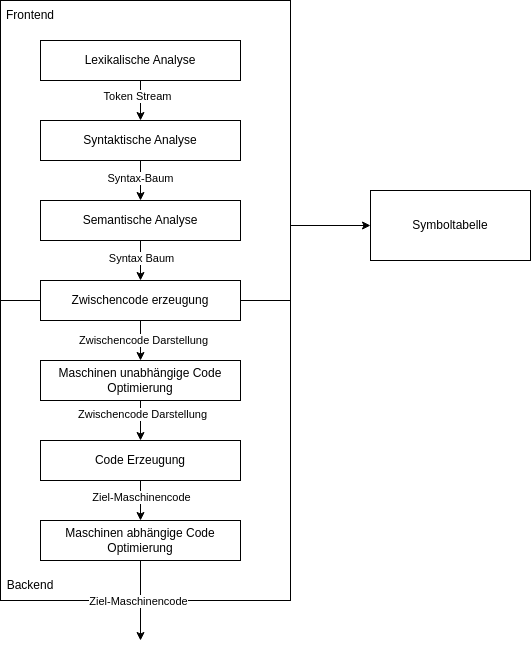
\includegraphics[scale=0.75]{compiler-ablauf-diagramm.png}
  \label{fig:compiler}
\end{figure}
\pagebreak
Abbildung ?.? zeigt eine Übersicht und das Ergebnis der einzelnen Phasen. Die Abbildung unterteilt den Ablauf wie eingangs beschrieben in Frontend und Backend.

In der ersten Phase teilt der Compiler den eingegebenen String in Tokens auf. Danach entsteht ein Syntaxbaum, der in eine Zwischencodedarstellung umgewandelt wird. Ab diesem Punkt beginnt das Backend des Compilers. Zuerst erzeugt es maschinenunabhängigen Code und anschließend maschinenabhängigen Code. Dieser maschinenabhängige Code ist auf dem zugrundeliegenden System ausführbar. (Compilers: Principles and Techniques, s. 30) 

%  Warum ein Transpiler?
Ein Compiler kann in unterschiedliche Art und Weise implementiert werden, wobei die Ausprägung der Prozessschritte, wie beispielsweise das Ergebnis der syntaktischen Analyse, häufig variiert. Es ergeben sich folglich Methoden den Compiler zu konstruieren.

Ein One-Pass-Compiler erzeugt keinen Zwischencode, sondern führt den Code direkt aus. Diese Methode wurde ursprünglich angewendet, um Speicherplatz zu sparen, da frühe Computer nur begrenzte Kapazitäten hatten und keine Zwischenergebnisse speichern konnten. Ein Beispiel für eine Sprache, die mit einem One-Pass-Compiler kompiliert wird, ist Turbo Pascal. (https://keleshev.com/one-pass-compiler-primer)

Diese Bauweise eines Compilers eignet sich nicht für den zu entwickelten Transpiler. Da es nicht das Ziel des Programms ist, den PL/I-Quellcode schnellstmöglich auf einem System in Binärcode umzuwandeln und auszuführen. Stattdessen liegt die Übersetzung im Vordergrund.

Eine weitere Methode einen Compilter zu entwickeln, ist ein Source-to-Source Compiler.
Dieser unterscheidet sich durch die Zielsprachen, in die er übersetzt. Während ein C-Compiler den C-Code nach der Zwischencodeerzeugung in Assemblersprache und anschließend der Assembler den C-Quellcode in Maschinencode übersetzt, wandelt ein Source-to-Source-Compiler beispielsweise C-Quellcode in Java-Zielcode um. 
Diese Vorgehensweise ist deckungsgleich mit der des entwickelten Transpilers. Lediglich das von der Hochsprache PL/I in die Hochsprache Java übersetzt wird.

Abbilding ?.? zeigt die Prozessschritte eine Transpilers.

\pagebreak
\begin{figure}[h]
  \centering
  \caption{Funktionsweise eines Transpilers}
  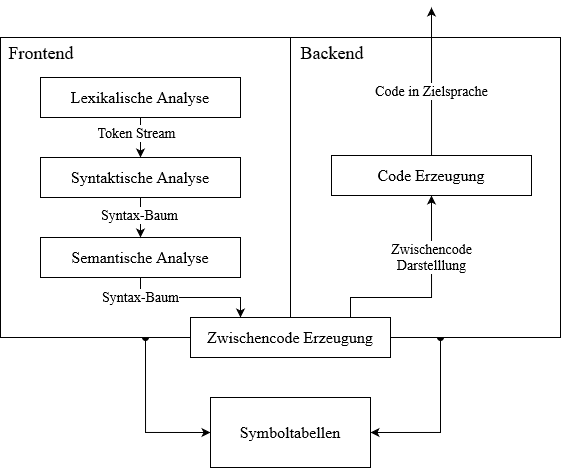
\includegraphics[scale=0.75]{transpiler-diagramm.png}
  \label{fig:transpiler}
\end{figure}
\pagebreak

Ein Vergleich von Abbildung ?.? mit Abbildung ?.? zeigt, dass die ersten Phasen bis zur Zwischencodeerzeugung gleich bleiben. In Abbildung ?.? sind jedoch die Prozesse des Frontends neben denen des Backends dargestellt. Diese Darstellung soll die unterschiede der Sprachebenen bei einem Transpiler und einem Compiler verdeutlichen.

Wie schon beschreiben übersetzt ein Compiler den Quellcode einer Hochsprache in eine maschinennahe Sprache wie Assembler. Ein Transpiler hingegen behält die Sprachebene der Quellsprache auch bei der Zielsprache bei. In Abbildung ?.? werden zudem die Phasen des Backends reduziert, da keine Übersetzung in eine maschinenabhängige Sprache erforderlich ist.

% @review
Deutlich wird auch der Unterschied zwischen Compiler und Transpiler, durch das Ergebnis der jeweiligen Übersetzung. 
Das Ergebnis der Übersetzung eines Compilers ist Binärcode der auf einem Zielsystem ausgeführt werden kann. Um hingegen das Ergebnis eines Transpilers auszuführen,
braucht es einen weiteren Compiler. Dieser Compiler muss den Zielcode der Zielsprache in Binärcode übersetzen und ausführen können.
Bei der übersetzung von PL/I-Quellcode zu Java-Zielcode, bedarf es also einen weiteren Java-Compiler der den Java-Zielcode in Binärcode übersetzt 
und damit ausführbar macht.  

% @review: Cross Compiler? - Hat hier eig nix zu suchen, ist Thema für Boostrapping aber nicht für Transpiler
Neben den Methoden der Konstruktion, gibt es auch unterschiedliche Verwendungen. 
Etwa existiert der Begriff der Cross-Kompilierung. Hierbei handelt es sich um die Möglichkeit einen Compiler, der sich auf einem externen Computersystem befindet zu verwenden um den Quellcode auf dem lokalen System in Binärcode zu übersetzen. (https://www.gnu.org/software/automake/manual/html_node/Cross_002dCompilation.html) 
Diese Verwendungsweise findet etwa Anwendung beim Bootstrapping. Liegt auf dem System noch kein Compiler für die Sprache vor, in der der Kernel geschrieben wurde, wird diese Methode verwendet um den Kernel-Code zu kompilieren. 
In dieser Arbeit kommt ein solcher Ansatz bedingt zum Einsatz. Wird der Transpiler in einem Webinterface verwendet, ist die Verhaltensweise ähnlich.
Da auch hier der Compiler auf einem anderen Host-Computer, den lokalen Quellcode übersetzt. Jedoch nicht in Binärcode. 
Der Transpiler lässt sich jedoch problemlos auch auf einem lokalen System verwenden. Bei einem Cross-Compiler, ist die komplitibiltät mit dem lokalen System von der Rechner-Architektur abhängig.

Sowohl One-Pass-Compiler, Transpiler bzw. Source-to-source Compiler als auch herkömmliche Compiler übersetzen das Programm basierend auf seiner Gesamtstruktur. (https://keleshev.com/compiling-to-assembly-from-scratch/excerpt-compiling-to-assembly-from-scratch.pdf)[S. 18ff.] 
Eine Alternative ist der Interpreter. Dieser führt den Quellcode direkt Zeile für Zeile aus.

% Wie arbeitet ein Interpreter?
Im Vergleich zu einem Compiler hat der Interpreter weder ein Frontend noch ein Backend. Es gibt keine klare Trennung zwischen einem Frontend, das eine unabhängige Repräsentation des Codes erzeugt, und einem Backend, das diese Repräsentation interpretiert. 

Programmiersprachen, die von einem Interpreter ausgeführt werden, sind beispielsweise PHP3, Ruby und JavaScript. Weiterhin wird ein Interpreter auch durch die Shell verwendet um Benutzerbefehle zu verarbeiten. Es ist auch möglich, sowohl einen Interpreter als auch einen Compiler für die Übersetzung bzw. Ausführung von Quellcode zu verwenden. Die Sprache 'Go' beispielsweise nutzt sowohl einen Compiler als auch einen Interpreter. Dabei wird das Go-Programm mit dem Befehl \verb+go build+ kompiliert und mit \verb+go run+ sofort durch den Interpreter ausgeführt. (https://craftinginterpreters.com/a-map-of-the-territory.html)
Um die Funktionsweise eines Interpreters besser mit der des Compiler zu vergleichen, soll die Verwendung eines Interpreters durch die Shell näher betrachtet werden. Eine Shell wird auf unixoiden und MS-DOS Betriebssystemen eingesetzt.
  
% Absatz: Ein Interpreter am Beispiel von Bash
Auf unixoiden Betriebssystemen dient die Shell als Interpreter für Skriptprogramme. Sie nimmt Benutzerbefehle direkt oder aus Skriptdateien entgegen und übergibt sie zur Ausführung an das Betriebssystem. Außerdem übernimmt sie die Ausgabesteuerung und kontrolliert die Datenströme. 
Um Befehle zu verarbeiten werden Interpreter Lösungen verwendet wie, \verb+bash+, \verb+csh+, \verb+zsh+ oder \verb+Powershell+.

% @review: Was unterscheidet die Shell von einem Übersetzer(Compiler)
Shell ist keine Programmier- oder Skriptsprache. Hingegen bringen die genannten Interpreter, Erweiterungen mit, die einer Programmiersprache ähneln. Bei \verb+bash+ werden etwa Programmiersprachen-ähnliche Konstrukte, wie Variablen, Kontrollstrukturen oder Funktionen verwendet. (https://www.gnu.org/software/bash/manual/bash.html#What-is-a-shell_003f)

In der Linux Manual Page wird \verb+bash+ auch als Command-language Interpreter bezeichnet. (https://www.man7.org/linux/man-pages/man1/bash.1.html)
Jedoch ist der allgemeine Zweck einer Shell immernoch die Verarbeitung von Befehlen und das ausführen von kompilierten Programmen.
Um den Unterschied zwischen einem Interpreter, wie bash, und einem Compiler zu verdeutlichen, wird in Abbildung ?.? die Arbeitsweise des Interpreters von bash dargestellt.

Abbildung 1.1 stellt den Ablauf der Skript-Interpretation dar.
\begin{figure}[h]
  \centering
  \caption{Ablauf der Interpretation eines Shell Programms}
  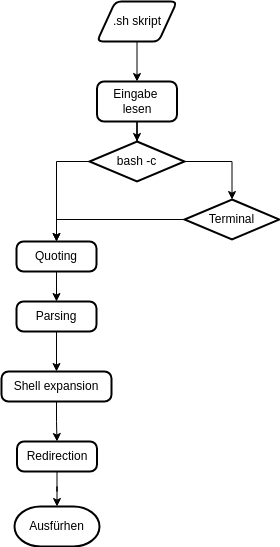
\includegraphics[scale=0.75]{shell_interpreter.png}
  \label{fig:shell}
\end{figure}
\pagebreak

Die Eingabe des Bash-Skripts wird zeilenweise gelesen, entweder über ein Terminal oder durch den Befehl \verb+bash -c+. Beide Eingabemethoden führen zur ersten Phase von Bash.

Die Phase das Quoting folgt dem Prinzip der lexikalischen Analyse, bei der alle Sonderzeichen entfernt werden, wie zum Beispiel Kommentare oder Backslashes. Sobald das Quoting abgeschlossen ist, entsteht ein String, der nur aus den Tokens eines Ausdrucks besteht.

Anschließend beginnt das Parsing, das der syntaktischen Analyse im Kompilierprozess ähnelt, jedoch keine Zwischencodeerzeugung beinhaltet. Hier wird lediglich zwischen einfachen Befehlen und zusammengesetzten Befehlen unterschieden. Einfache Befehle umfassen das Ausführen der integrierten Shell-Programme wie \verb+ls+, \verb+wc+ oder \verb+mkdir+. Zusammengesetzte Befehle bringen zusätzliche Logik in das Bash-Skript ein, wie zum Beispiel \verb+if+, \verb+while+ oder \verb+case+.

Der Verarbeitungsprozess setzt sich mit der Shell-Expansion fort, bei der in einem Befehl eingebettete relative Ausdrücke durch ihre absoluten Repräsentationen ersetzt werden. Zum Beispiel würde im Ausdruck \verb+echo ${pwd}+ das \verb+$pwd+ durch den absoluten Pfad des aktuellen Verzeichnisses ersetzt.

Schließlich wird der des ausgeführten Skripts durch die \verb+stdio+-Bibliothek ausgegeben, in der Kommandozeile ausgegeben.
(https://www.gnu.org/software/bash/manual/bash.html#Shell-Operation)

% Absatz: Zusammenfassende Unterscheidung zwischen Interpreter und Transpiler, Was sind gemeinsamkeiten und unterschiede von Transpiler und interpreter?

Zusammenfassend zeigen sich sowohl Ähnlichkeiten als auch Unterschiede zwischen einem Interpreter und einem Compiler. Beide durchlaufen die Phasen der lexikalischen und syntaktischen Analyse, wobei sie den Quellcode zunächst bereinigen, um Kommentare, Leerstellen oder andere für die Übersetzung irrelevante Symbole. Anschließend erfolgt entweder die direkte Übersetzung des Quellcodes oder die Erzeugung einer unabhängigen Repräsentation.

% Der entscheidende Unterschied liegt darin, dass der Interpreter den Quellcode lediglich zeilenweise direkt übersetzt, während der Compiler das Programm in eine andere Form transformiert und liest. Dabei stehen die verwendeten Ausdrücke des Eingabecodes in Beziehung zueinander, beispielsweise durch die Verschachtelung von Verzweigungen und Schleifen.

In diesem gesamten Prozess werden ausschließlich Bash-Befehle verwendet. Der Quellcode wird nicht von einer Hochsprache in eine Assamblersprache oder eine andere Hochsprache umgewandelt. Dies verdeutlicht einen zentralen Unterschied zwischen einem Interpreter und einem Compiler: Es entsteht keine Repräsentation des Codes in einer anderen Sprache. Vom lesen des Quellcodes bis zum ausführen des Programms bleibt der Interpreter bei einer Sprache. 

Um PL/I-Code korrekt in Java zu übersetzen, sind Verbindungen zwischen den Ausdrücken wichtig. Eine bloße zeilenweise Übersetzung könnte zu einem Java-Programm führen, das kaum objektorientierte Paradigmen enthält. Der Transpiler sollte eine solche Repräsentation darstellen können.
Allgemein sei zu erwähnen das es möglich ist einen Interpreter für die Übersetzung zu verwenden, dies ist jedoch nicht Bestandteil dieser Arbeit.

Wie schon in den Abbildungen ?.? und ?.? dargestellt sind die ersten Arbeitsschritte des Transpilers die lexiklaische und syntaktische Analyse.
Für beide Prozesschritte werden ein Parser und Lexer benötigt. Mit einem Compiler-Compiler können diese Module mit einer formalen Grammatik generiert werden.
Das folgende Kapitel beleuchtet Grammatiken formaler Sprachen wie PL/I und Java genauer.

% - Erweiterung des Umfangs während der Laufzeit
% - Trennung Laufzeit/Konzeptionsphase

% - Hier erwähnen das eine geminsamkeit die definition von Grammatiken ist, dann überleiten zu Formale Grammatiken.
% - Auch Entscheidung treffen was genau der Transpiler ist, Compiler oder Interpreter
\pagebreak
   
   
\subsection{Formale Sprachen und ihre Grammatiken}
% Warum braucht ein Compiler eine Grammatik?
In dem vorangegangen Kapitel wurden unterschiedliche Methoden, Anwendungsgebiete und Formen der Sprachinterpretation eines Computers vorgestellt. Damit die Interpretation von Sprachen korrekt erfolgt, braucht ein Computer Regeln. Grammatiken beinhalten diese Regeln. Damit der Transpiler korrekt arbeitet wird eine definierte Grammatik benötigt. Nur so können die Prozessschritte der Lexikalischen- und der Syntatkischen Analyse korrekt erfolgen. Denn diese Schritte prüfen den eingegeben Quellcode auf seine grammartikalische Richtigkeit. Bevor also die Sprachliche Analyse erfolgen kann, sollte eine Grammatik angwendet werden.
	
% Woraus besteht eine Grammatik?
Um eine Grammatik anzuwenden muss klar sein, um welche Grammatik es sich handelt. Weiterhin sollte bestimmt werden welche Art von Sprache beschrieben werden soll. 
Eine formale Sprache unterscheidet sich von einer natürlichen Sprache in der Anwendungsform. Die Anwendung von solchen Sprachen dient der logisch präzisen Beschreibung von Ausdrücken. (introduction to formal languages and automata, S. 149ff.) Eine Grammatik besteht aus Variablen, Terminalsymbolen, einen Startsymbol und einer Produktion. Zusammengefasst in:

\begin{center}
\begin{equation}
G=(V,T,S,P)
\end{equation}
\end{center}

Hierbei \verb+V+ für Variablen bzw. Nicht-Terminalsymbole, \verb+T+ für Terminale, \verb+S+ für Start und \verb+P+ für Produktion steht. Dabei ist \verb+S+ ein Teil von \verb+V+. (introduction to formal languages and automata, S. 31ff.)


% @review: Keine Hierachie Einordnung, ledilgich nennen das es sie gibt.
% Welche Typen von Grammatiken gibt es? Chomsky Hierarchie
Grammatiken lassen sich weiter durch die Chomsky Hierarchie spezifizieren. Noam Chomsky unterteilt Grammatiken in vier Ebenen. Ebene null beschreibt unbeschränkte-, Ebene eins kontextsensitve-, Ebene zwei kontextfreie- und Ebene drei reguläre Grammatiken.(https://hpi.de/friedrich/teaching/units/grammatiken.html) 

\pagebreak

Um eine Grammatik darzustellen werden Ableitungen von Produktionen verwendet. In Listing ?.? ist die Produktion einer einfachen \verb+if+ und \verb+else+ Verzweigung dargestellt.

% @todo: PL/I Verwenden und Kontext herstellen
\begin{center}
\begin{equation}
S \to \mathbf{if}\: expr\: \mathbf{then}\: stmt\: \mathbf{else}\: stmt\: | \mathbf{if}\: expr\: \mathbf{then}\: stmt;
\end{equation}
\begin{equation}
expr \to expr\: op\: term\: | term
\end{equation}
\begin{equation}
op \to \mathbf{>}\: |\: \mathbf{<}\: |\: \mathbf{=}\: |\: \mathbf{!}
\end{equation}
\begin{equation}
term \to term\: multOp\: factor\:
\end{equation}
\begin{equation}
factor \to \mathbf{id}\: |\: \mathbf{constant} 
\end{equation}
\end{center}
 
Mit der beschriebenen Grammatik ist folgender Ausdruck zulässig.

\begin{verbatim}
IF A > B THEN 
	CALL proc_1;
ELSE 
	CALL proc_2;
END
\end{verbatim}

Nicht zulässig ist hingegen.

\begin{verbatim} 
CALL IF THEN A > B proc_1;
\end{verbatim}

% @todo: Beispiel-Parsebaum analyse, https://en.wikipedia.org/wiki/LR_parser 
	
% Wie werden Grammtiken in einem Transpiler Programm verwendet?
Die bisher definierten Grammatiken sind in dem Sinne von Bedeutung, weil die Lexikalische und Syntaktische Analyse des Transpilers aus einer solchen Grammatik erzeugt werden. Mithilfe eines Compiler-Compilers kann aus einer repräsentation einer formalen Grammatik ein Parser definiert werden.
 
Für den PL/I-Transpiler bedeutet, dass die aktuelle PL/I-Grammatik für den Parser definiert werden muss. Die aktuellste Grammatik wird durch IBM, in der PL/I Language Referenz definiert. Aus dieser wird mithilfe von JavaCC ein Parser erzeugt. Weshalb in dem folgenden Kapitel 1.5 der Compiler-Compiler und die dazugehörige Grammatik näher beschrieben wird.

% - Theoretischer Abriss
% - Einordnung der resultate der PA 4
%- PL/1 Syntax Wo zu finden? Welche Version der Sprache? 
%	- Reguläre Ausdrücke Syntax, Beispiel einer Grammatik die ich mit verwende, Typ einer Grammatik
%  - Literatur
%    - Chomsky Hierarchie Bücher
%    - https://www-igm.univ-mlv.fr/~berstel/LivreCodes/Codes.html
%  - Woraus besteht eine Grammatik?
%   - Wie lassen sich Grammatiken der Komplexität nach anordnen?
%  - Chomsky Hierarchie
%  Erst Chomsky Hierachier, dann nach Komplexität einordnen und am Beispiel von Regulären Ausdrücken und PL/I Grammatik einführen.
     
\subsection{Anwendung von Formalen Grammatiken in JavaCC}
% 1. Was ist ein Compiler-Compiler? (Verbindung von formalen Grammatiken zu JavaCC)

Nachdem in formale Grammatiken eingeführt wurde, soll nun näher beschrieben werden welche Rolle diese in der Entwicklung des Transpilers spielen.

Der Lexer der die lexikalische Analyse und der Parser, der die Syntaktische Analyse durchführt werden durch JavaCC erzeugt. 
JavaCC ist ein Compiler-Compiler der aus einer formalen Grammatik einen Lexer und einen Parser generiert. 
In Kapitel 1.3 wurde bereits in die Thematik der formalen Grammatiken eingeführt, in diesem Kapitel wird nun die praktische implementation dieser Grammatiken im Zusammenhang mit dem Transpiler beschrieben.

Ein Compiler-Compiler ist eine Technologie mit der aus einer formalen Beschreibung einer Grammatik ein Lexer und ein Parser erzeugt werden. 
Der Lexer und der Parser wenden die in der Grammatik definierten Regeln an und verarbeiten entsprechend die übergebenen Ausdrücke.
Die Darstellung der Grammatik erfolgt in der Regeln in einer Art erweiterten Backus-Naur-Form (EBNF). 
Beispielhafte Compiler-Compiler sind neben JavaCC, Yacc, Antlr und Lexer.
In Kapitel 1.3 wurde bereits vereinfacht eine Produktion aus der PL/I-Grammatik dargestellt. Ähnlich erfolgt auch die Darstellung in einer Grammatikdatei. Folgendes Beispiel zeigt die Darstellung eines \verb+IF ELSE+ Ausdrucks. 
(https://javacc.github.io/javacc/)

\begin{verbatim}
void if_statement() #IF :
{}
{
  < IF > bool_expression() (bool_operation() bool_expression() )*
  < THEN >proc_body()
  [< ELSE >
  	proc_body()]
  	
}
\end{verbatim}

In JavaCC besteht die Möglichkeit die Beschreibung von Produktionen in Methoden zu Kapseln.
In Zeile 1 ist der Methodenkopf zu sehen. In diesem Fall erzeugt die Methode \verb+if_statement+ keinen Rückgabwert.
Das durch die Raute gekennzeichnete Symbol ist die Repräsentation im Parsebaum und zusätzlich auch die Darstellung im Zwischencode.
Im Körper der Methode wird der If-Ausdruck weiter definiert. Terminalsymbole werden in der JavaCC Grammatik mit den größer-als und kleiner-als Zeichne umrandet. Die Nicht-Terminalsymbole hingegen sind wie im Listing ?.? dargestellt weitere Methoden, die wiederum weitere Ausdrücke beschreiben.
Ähnlich wie bei der Produktion aus Listing ?.?, so lange bis lediglich Terminalsymbole übrig bleiben.
Die Methode \verb+bool_expression+ etwa, beschreibt einen zulässigen Boolschen Ausdruck, der durch einen weiteren boolschen Operator mit einem weiteren booleschen Ausdruck verknüft werden kann.
Letzter Ausdruck, kann Leer sein und beliebig oft wiederholt werden. Das ermöglicht komplexe boolsche Operationen.

Weiterhin wird in der Methode \verb+proc_body+ beschrieben welche Ausdrücke in dem Verzweigungskörper zulässig sind. Dazu zählt bspw. auch eine weitere \verb+IF ELSE+ Verzweigung. So werden auch verschachtelte Ausdrücke möglich.
Werden nach und nach die Methoden durch den Compiler-Compiler aufgerufen, ergibt sich eine Regel für Verzweiguns-Ausdrücke. Nach diesem Prinzip ist die gesamte Grammatik gestaltet. 
Die Wurzel aller Methoden, die einen Ausdruck beschreiben, ist dabei die Wurzel Methode \verb+program+, welche das gesamte Programm darstellt. Eine solche Kapselung macht die Grammatik übersichtlich.
Aus dem definierten Ausdruck aus Listing ?? wird schlussendlich ein Parsebaum erzeugt, der durch die Module des Transpilers weiter verarbeitet wird.

% Warum ein Compiler-Compiler verwenden?

Ein Compiler-Compiler generiert somit einen fertigen Parser, aus einer Datei in der eine Grammatik beschrieben wird. Nun gibt es auch die Möglichkeit einen Parser und Lexer selbst zu programmieren. In der Version aus der Projektarbeit-4 wurde ursprünglich ein selbstgeschriebener Lexer verwendet.
Jedoch birgt dieses Vorgehen einen Nachteil. Die Grammatik für den Transpiler ist an zwei stellen definiert und muss somit auch an zwei Stellen gewartet werden.
Wird in die Grammatikdatei für den Parser ein neuer Ausdruck hinzugefügt, muss dieser Ausdruck auch durch den Lexer verarbeitet werden können.
Ursprünglich musste so der Lexer angepasst werden und die Grammatikdatei für den Parser. 
Das führte zu einem erhöhten Arbeitsaufwand und Fehleranfälligkeit. Schlussendlich wurde der selbstgeschriebene Lexer entfernt und der von JavaCC definierte Lexer verwendet.
Somit ist ein Compiler-Compiler gut dazu geeignet den Arbeitsaufwand für die Entwicklung eines Compilers, bzw. eines Transpilers zu reduzieren. 
Es lohnt sich auch bei der Entwicklung auf bereits definierte Resourcen zurückzugreifen. 
Grammatiken für Cobol und Java wurden bereits von der JavaCC Community bereitgestellt. (https://javacc.github.io/javacc/)
Im Fall von PL/I ist keine Grammatik vorhanden. Weshalb bei der Entwicklung des Transpilers, die IBM Language Reference für PL/I die Hauptquelle für die Grammatikdatei ist.   

% @todo: Beschreibung hinzufügen
\begin{tabular}[h]{l|c|r}
Klasse & Beschreibung \\
\hline
JJTPl1ParserState.java & ... \\
Node.java & ... \\
ParseException.java & ... \\
Pl1Parser.java & ... \\
Pl1ParserConstant.java & ... \\
Pl1ParserTokenManager.java & ... \\
Pl1ParserTreeConstants.java & ... \\
SimpleCharStream.java & ... \\
SimpleNode.java & ... \\
Token.java & ... \\
TokenMgrError.java & ... \\
parser.jjt & ... \\
\end{tabular}


JavaCC generiert dynamisch den eigentlichen Parser, hier Pl1Parser, den TokenManager und die ParserConstants Klasse. Die restlichen Klassen sind Boilerplate-Code und werden bei jeder Grammatik generiert. Diese werden auch nur beim initalen kompilieren generiert. Eine weitere Erläuterung des Prasers für den Transpiler ist in Kapitel ?.?

% Wie wird JavaCC in die Entwicklung des Transpiler eingebunden ? (Hinleitung zur Architektur beschreibung)
Durch die Verwendung des JavaCC Jjtree-Moduls, kann global innerhalb des Projekts auf den Parse-Baum zugegriffen werden. 
Der Prase-Baum wird unteranderem durch die Module verwendet, die die Semantische-Analyse und -Synthese repräsentieren.
Erst durch diese wird der Java-Code erzeugt.
Ebenfalls wird für den Parser ein File-Stream benötigt, ein Scanner liefert solchen.
Neben den Parser werden also weitere Module verwendet um schlussendlich den Java-Code für den Benutzer bereitzustellen.
Die gesamte Architektur des Transpilers und dessen weitere Module wird in dem nachfolgenden Kapitel betrachtet. 
Hier werden auch die Technologien vorgestellt die neben JavaCC verwendet werden. 

\section{Technisches Vorgehen}
\subsection{Techstack}
%- Compiler Compiler -> JavaCC: Integration in das Projetk, Grund für die Wahl der Technologie
In Kapitel 1.4 wurde bereits mit JavaCC eine Technologie vorgestellt. Neben JavaCC kommen auch weitere Technologien während der Entwicklung zum Einsatz. In dem folgenden Kapitel werden die weiteren verwendeten Technologien, während der Entwicklung des Transpilers, vorgestellt.

%- Programmiersprache -> Java: Integration in das Projekt, Grund für die Wahl.
Allgemein wurde der Transpiler in der Programmiersprache Java entwickelt. 
Die Entscheidung für Java ist auf fundierte Fachkenntnis und erweitereten Erfahrungswerten zurückzuführen. Weiterhin zählen die Vorteile die in Kapitel ?.? für Java erwähnt wurden, ebenso in diesem Fall.
Den Administratoren soll auch die Möglichkeit gegeben werden, Module einfach auszutauschen. Mithilfe von Objektorientierten Paradigmen, lässt sich eine lose Kopplung der Klassen realisieren und damit eine Modulare Bauweise des Software Projekts.
Einhergehend fiel die Wahl auf JavaCC aufgrund der Entscheidung für die Entwicklung des Transpilers in Java. Eine alternativer Compiler-Compiler für Java, ist Antlr. 

%- IDE -> Eclipse: Integration in das Projekt, Grund für die Wahl.
Der Java-Quellcode des Transpilers wurde in Eclipse geschrieben. Die IDE Eclipse ermöglicht eine kostenlose Entwicklung, Verwaltung, Überprüfung und Kompilierung von Java Software-Projekten. Weiterhin bietet Eclipse eine breite Software-Repository an Plugins an um die Funktionalität der IDE zu erweiteren. Dadurch ist eine integration von JavaCC in die IDE möglich und erleichtert die Entwicklung des Parsers ebenfalls. Ein weiterer Grund für die Entscheidung für JavaCC. Alternativen zu Eclipse, können etwa IntelliJ oder Visual Studio Code sein. 

%- Maven -> Dependency Management: Integration in das Projetk, Grund für die Wahl der Technologie
Die Version aus der Projektarbeit-IV des Transpilers nahm die Native Projektstruktur von Eclipse als Vorlage. Diese Projektvorlage brachte jedoch negative Aspekte mit sich. Es war nötig JavaCC manuell zu installieren und einzurichten. Zusätzlich mussten Pfadvariablen im Quellcode angepasst werden. Das erschwerte den Benutzern den Zugang zu dem eigentlichen Projekt.
Zurückzuführen ist dies auf die fehlenden Software-Abhängigkeitsverwaltung. In der Ursprünglichen Version des Transpilers musste der Benutzer selbst herausfinden welche Software dieser benötigt um das Programm zu starten. Dieser Umstand ergibt eine Hürde, welche den Einstieg in die Umwandlung erschwerte. 

Dieses Problem wurde gelöst in dem das Software-Projektmanagement-Werkzeug Maven eingesetzt wurde. Maven löst mithilfe des Project-Object-Model (POM) Abhängigkeiten. 
Dadurch werden Benutzer und Administratoren bei dem Buildprozess entlastet.
Ein weiterer Vorteil den Maven liefert ist die vordefinierte Projektstruktur. Mavens Projektstruktur liefert zwei gespiegelte "src" Ordner, welche je den Quellcode enthalten und die dazugehörigen Tests.
Auch hier finden sich Benutzer und Administartoren leichter zurecht.

%- Testing -> JUNit Tests: Integration in das Projetk, Grund für die Wahl der Technologie

Zum Testen der Anwendung wurde das Java-Testing Framework JUnit 5 verwendet. Es wurden für jede Klasse zugehörige Test-Klassen geschrieben. In den Test-Klassen wurde komplexere Methoden isoliert getestet.
Die Wahl von JUnit ist begründet durch die einfache Handhabung, der kompatibilität mit der IDE Eclipse und dem Projektmanagement Werkzeug Maven. Weiterhin ist JUnit mit eines der bekanntesten Unit-Testing-Frameworks für Java-Quellcode. Alternativen wären etwa gewesen TestNG oder mockito. (https://testng.org/ & https://site.mockito.org/).
Genaueres bezüglich des Testings des Transpilers ist in Kapitel ?.? nachzulesen.

%- Platform -> Spring

Mithilfe der, in diesem Kapitel genannten Software-Werkzeuge, wurde der Transpiler entwickelt. Die Entwicklungsphase folgte jedoch nach der Konzeptionsphase.
In der Konzeptionsphase wurde die Architektur der Anwendung ausgearbeitet und später in Quellcode realisiert. 
Dieses Vorgehen wurde in der Projektarbeit-IV nicht verfolgt, was zu einigen Problem führt. Diese Probleme zeigt sich in der mangelnden Qualität und der nicht Benutzerfreundlichen Umgebung der Anwendung.
Aus diesem Grund wird in dem nächsten Kapitel zuerst das Architekturbild beschrieben, woraufhin genauer auf den Quellcode der Anwendung eingegangen wird.

\subsection{Architektur} 

Die Architektur des Transpiler wurde nachdem Vorbild eines Model-View-Controller (MVC) Konzept entworfen. 
Es wurden Module definiert die zum Bereich des Models gehören. Etwa solche wie die Symboltabelle, oder Templates für Java-Zielcode.
Der Controller entspricht jeglichen Modulen, die den PL/I-Quellcode analysiere, verarbeiten und schlussendlich in den Java-Zielcode übersetzen.
Dem View wurden jeglich Module zugesprochen, die den Benutzer eine Interaktion mit dem Transpiler ermöglichen.

% @todo Wie benutze ich den Transpiler?
Der Benutzer oder der Administrator kann mit der Ausgewählten Schnittstelle interagieren und so den Transpiler benutzen. Eine Schnittstelle, ist entweder über die IDE in 
der das Projekt importiert wird oder die Kommandozeile.

% Was ist das Ziel der Architektur?
Um den Administratoren die Möglichkeit zu gewährleiste Module auszutauschen und anzupassen sollte die Architektur des Transpilers eine lose Kopplung der Module aufweisen.
Zusätzlich sollten die Benutzer auf Fehlermeldungen reagieren können.
In Abbildung ?.? sind die Module in dem Ablauf des Transpilers dargestellt.

\begin{figure}[h]
	\centering
	\caption{Der Aufbau des Transpiler}
	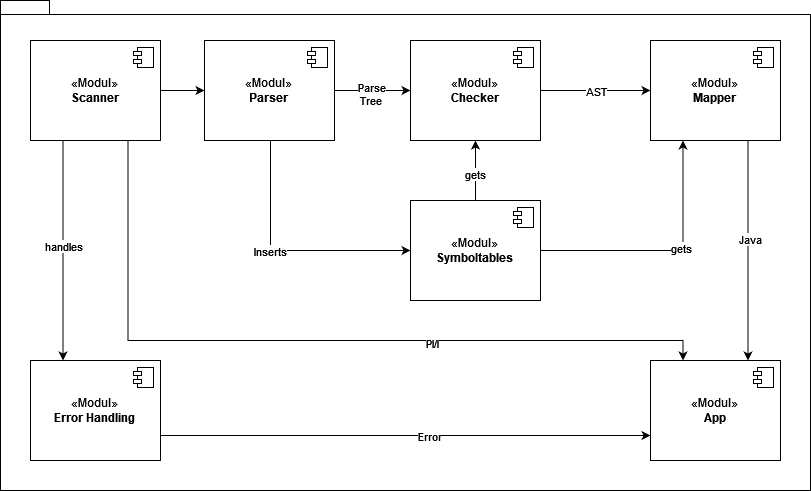
\includegraphics[scale=0.75]{AbstraktesUML_1.png}
	\label{fig:modules}
\end{figure}

% Wie sind die Module momentan gebaut?
% App Modul
Die Verarbeitung des PL/I-Quellcodes beginnt mit dem App-Modul. Das App Modul ist die Schnittstelle für alle weiteren Module. Ein Modul kann durch die Instanziierung der Hauptklasse des Moduls eingefügt werden. Entfernt wird das Modul durch das Löschen der Instanz. Das Modul beinhaltet auch die \verb+main+ Methode.

Der Scanner wird als erstes Instanziiert. Dieser liest aus der Config-Datei den Pfad der \verb+pli+ Datei, die übersetzt werden soll. Die Datei wird als \verb+InputStream+ an den Parser übergeben.

Der durch JavaCC erzeugte Parser wird ebenfalls in dem App-Modul instanziiert. Dieser behandelt den PL/I-Quellcode entsprechend der definierten Grammatik. Hier wird die Lexikalische und Syntaktische Analyse realisiert.

Während des parsings werden Variablen-, Prozeduren-, oder Packagebezeichner des PL/I-Quellcode, in die Symboltabelle eingefügt. Diese wird in dem Parser Modul zum ersten mal instanziiert. 

Das Ergebnis des Parsers ist ein Parsebaum.
Ist der Parsebaum erstmal entsprechend erzeugt, wird dieser weiterhin durch das Checker Modul verarbeitet. In diesem Modul wird die semantische Analyse des Quellcodes durchgeführt. Dabei wird auch die Symboltabelle verwendet um die Referenzen der Bezeichner im Quellcode auf korrketheit zu überprüfen. Teilweise ist es notwendig den Parse-Baum umzustellen. Ist der Parsebaum korrekt, oder korrekt verarbeitet worden, kann dieser als Abstrakter-Syntax-Baum (AST) im Mapper-Modul verwendet werden.

% @review: Hier erwähnen wie Configdatei bzw. Scanner den Ausgabe Ordner beeinflussen wenn das implementiert wurde.
Das Mapper-Modul repräsentiert die Synthese des PL/I-Quellcodes in Java-Zielcode. Der AST wird hier Stück für Stück abgearbeitet und mit entsprechenden Java-Ausdrücken übersetzt. Schlussendlich wird in dem \verb+target+ Ordner das übersetzte Programm abgelegt.
 
Ist das Programm fertig übersetzt kann der Java-Zielcode und die nötigen Klassen aus dem target Ordner exportiert werden und kompiliert, bzw. gewartet werden.

% @todo: Wie sind Module zueinander abhängig?
Die Abhängigkeit sollte nachdem Zielbild der Architektur möglichst gering gehalten werden.
Deshalb wurde das App-Modul hauptsächlich verwendet um die Komponente zu integrieren und gemeinsam zu verwenden.
Etwa das Scanner Modul für über einen Parameter durch das Parser Modul verwendet.
Es bleibt jedoch nicht aus Module auch außerhalb des App Moduls, in andere Module zu integrieren.
Bei der Symboltabelle ist das der Fall. Die Symboltabelle wird einerseit von dem Parser Modul verwendet und andereseits von dem Mapper Modul.
Dadurch muss auch in beiden das Symboltable Modul instanziert werden. Um einen Überblick über abhängigkeiten zu verschaffen, zeigt
Abbidlung ?.? aktuell die Beziehungen der Module untereinander, ohne dabei detailierter auf Klassenhierachien einzugehen. 
Eine Detailbetrachtung der Anwendung soll in Kapitel ?.? erfolgen.

\begin{figure}[h]
	\centering
	\caption{Die Abhängigkeiten der Module}
	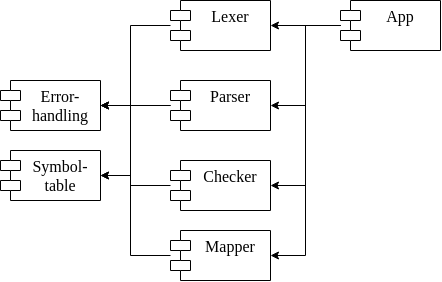
\includegraphics[scale=0.75]{Beziehungen_Modules.png}
	\label{fig:modules}
\end{figure}

Zu erkennen ist in Abbildung ?.? das die Abhängigkeiten unter den Modulen eine Kaskade Form aufweisen.
Diese Form hat den Vorteil das Module aus dieser Kette verändert werden können ohne Vertikal verlaufende Module direkt zu beinträchtigen.
Dennoch ist an dieser Stelle zu erwähnen das kein Modul isoliert betrachtet werden darf. Denn eine Veränderung eines Moduls bedeutet das auf Horizontaler 
Ebene die Verarbeitung verändert wird.
Jedes Modul gibt die Ergebnisse weiter an das nächste bis ein tatsächlicher Zielcode entsteht, oder eine Fehlermeldung.
Somit würde etwa das Modul Lexer verändert werden, so muss auch in App diese Veränderung berücksichtigt werden.
Würde etwa in der Symboltabelle ein PL/I-Symbol gelöscht, hätte dies Auswirkungen auf jegliche Module auf Horizontaler Ebene. 

% Wie sind die Module momentan gebaut?
Der Aufbau der Module ist dabei durch Klassen spezifisiert. Jede Klasse bietet eine Sammlung von Methoden zur Lösung eines Problems,
oder zu bereitstellung von Ressourcen. 
Wie schon in Kapitel ?.? erwähnt gehört zu jeder Klasse eine Test-Klasse. Neben den Klassen existieren Interfaces und Enums in den Modulen,
die erneut Resource bereitstellen.

% @todo: Wie wird es erweitert?
Der Administrator kann die Module um Klassen, Interfaces, Enums und weiteres erweiteren oder ersetzen.
Dabei sollte jedoch die Eingangs beschriebene Kaskdierung der Module untereinander berrücksichtigt werden.
Entscheidet sich der Administartor dazu etwa eine Methode zu entfernen und eine selbstentwickelte zu verwenden, ist ledligch die bisherige 
referenz zu ersetzen, welche in dem App Modul in der App Klasse aufzufinden ist.
In der vorherigen Version des Transpilers wurde etwa die Lexer-Klasse entfernt und die Klassen des Compiler-Compilers verwendet.
Der Quellcode des Lexer besteht jedoch und ist lediglich als Deprecated markiert. Die erneute Verwendung des Lexer würde über den Aufruf der Methode in Main erfolgen.
Hingegen wären hier weitere Schritte notwendig, wie etwa das einfügen einer temporären Datei, die von dem Parser als InputStream entgegen genommen wird und weiter verarbeitet wird.

Nachdem nun die Module deutlich beschrieben wurden, soll nun in Kapitel ?.? eine Detailansicht des Transpilers erfolgen.
Ab diesem Punkt soll genauer auf den Quellcode eingegangen werden um nachzuvollziehen wie der Transpiler, den PL/I-Quellcode
in Java-Zielcode umwandelt.

%Bausteine
%- Software Architektur
	%- Planen mithilfe eines UML
	%- UX Design 
    %    - zweite Diagramm, des Benutzerfluss
    %    - wie Benutzung abläuft
	%	- Website?
	%	- Docker Container?
%- Fehlertracking
%- Struktuierung des Programms, sodass ein Benutzer es selbständig erweitern kann

%\subsection{Aspektorientierte Programmierung}
%- Wie funktioniert Aspektorientiert Programmierung?
%	- Wie Löse ich mit Aspektorientierter Programmierung konkrete Probleme?
%- JavaBeans
%- Spring
%	- Wie setzt Spring Aspektorientierte Programmierkonzepte ein?
 
\subsection{Module des Transpilers}
Die Module des Transpilers repräsentieren je einen Verarbeitungsschritt.
In diesem Kapitel sollen die Module nach ihrer Verarbeitungsreihenfolge vorgestellt werden.
Dabei soll ein UML-Diagramm je zu beginn der Unterkapitel verdeutlichen wie die Klassen
in den Modulen zueinander aufgebaut sind. In jedem Diagramm wird auch auf die Einbindung in die App-Klasse
 eingegangen.
Die Beschreibung beginnt mit dem Scanner.

\subsubsection{Der Scanner und Parser}
\paragraph{Scanner}
Wie Kapitel 1.? eingeführt wird der Parser vollständig durch JavaCC generiert.
Damit der Parser den PL/I-Quellcode in eine Zwischencode Darstellung übersetzen kann,
braucht dieser eine PL/I-Datei, die als Stream Übergeben wird.
Den Pfad zu der Datei gibt der Administrator in der Konfigrationsdatei an.
Das Modul Scanner liest die Konfigurationsdatei und versorgt den Parser mit notwendigen Resourcen.
Abbildung ?.? zeigt das UML-Diagramm des Scanner Moduls.

\begin{figure}[h]
	\centering
	\caption{Das Scanner Modul}
	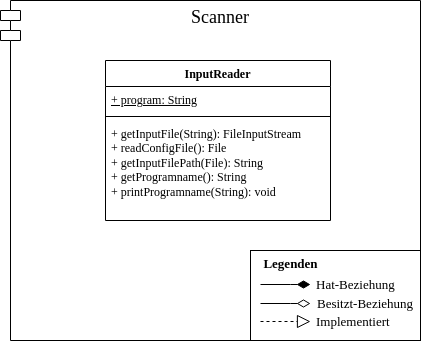
\includegraphics[scale=0.75]{scanner-klasse-uml.drawio.png}
	\label{fig:Scanner Modul}
\end{figure}

Das Scanner Modul besteht aus den Klassen \verb+InputReader+ und \verb+Lexer+. 
Die \verb+InputReader+ Klasse liest die Konfigurationsdatei ein und speichert den Pfad, der mit der Variable \verb+PATH+
hinterlegt ist. Ein Ausschnitt einer möglichen Konfigurationsdatei ist in Listing ?.? hinterlegt.

\begin{verbatim}
	PATH=./src/main/java/res/pli/NPP1NFG.pli;
\end{verbatim}

Die Methode \verb+getInputFilePath+ gibt den Pfad der PL/I-Quellcode Datei als String zurück.
Dieser String wird beim Aufruf der \verb+getInputFile+ Methode benötigt, um aus der Datei einen \verb+InputStream+ zu erzeugen.
Mithilfe des InputStreams kann dann die Datei als Parameter an den Parser in der Klasse \verb+App+ im Modul \verb+App+
übergeben werden. 


\paragraph{Lexer}
Die Klasse Lexer des Moduls Scanner enthält den ehemals selbst geschriebene Lexer für die lexikalische Analyse. Dadurch das dieser Prozess nun vollständig von dem JavaCC-Parser übernommen wird, wurde die Methode \verb+getToken+ überflüssig. Diese ist als veraltet mit der Kennung 'Deprecated' beschrieben, sie kann im Projekt noch verwendet werden, jedoch mit einem Risiko das die Ergebnisse der Methode nicht korrekt sind. 
Zu einem späteren Zeitpunkt ist denkbar den selbstgeschriebenen Lexer zu optimieren und erneut einzubinden. Weshalb dieser nicht gelöscht wurde. 
Weitere Methoden in dieser Klasse werden ebenfalls nicht länger von Klassen aus anderen Modulen verwendet. 

\paragraph{Parser}
Das Parser-Modul deckt somit die lexiklaische und die syntaktische Analyse des PL/I-Quellcodes ab.
Wie schon in Kapitel 1.4 erwähnt werden jegliche Klassen des Prasers durch die \verb+.jjt+ Grammatikdatei 
generiert. Da diese Klassen sehr umfangreich sind, werden diese in Abbildung ?.? lediglich in Abgekürzter Form dargestellt. 

\begin{figure}[h]
	\centering
	\caption{Das Parser Module}
	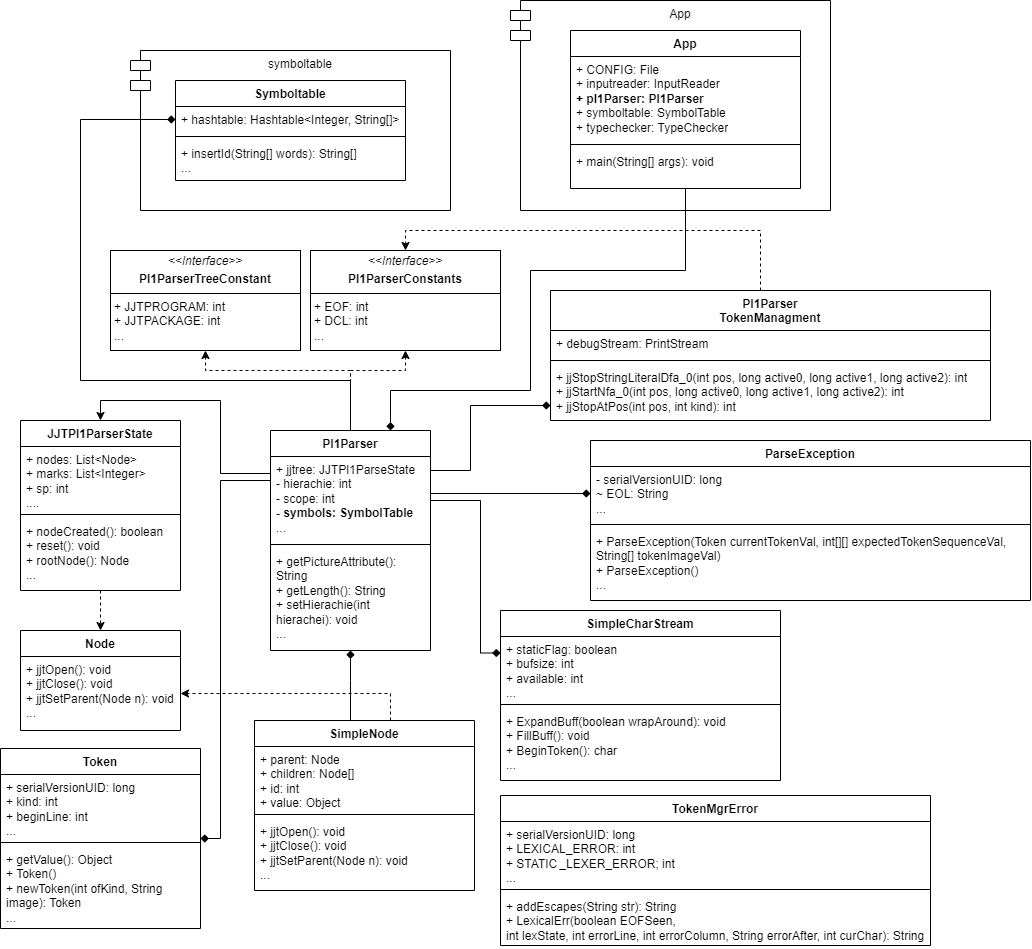
\includegraphics[scale=0.75]{parser-module-uml.drawio.png}
	\label{fig:Parser Module}
\end{figure}

Der Parser wird über die Klasse \verb+Pl1Parser+ in dem App Modul instanziert. In der Parser-Klasse sind auch jegliche manuell geschriebenen Methoden aus der Grammatikdatei integriert. 
Dazu gehören etwa die Methode \verb+installId+, sowie Getter und Setter-Methoden für benötigte Attribute eines Parsbaum-Knotens. 
Etwa für die Variable \verb+scope+, die beschreibt, ob eine Variable global oder lokal initialisiert wurde, kann der Wert über die implementierten Getter- und Setter-Methoden abgerufen werden.
Die ebenfalls in der Grammatikdatei definierten Tokens werden in der Klasse \verb+Pl1ParserConstants+ als Konstanten definiert. Wobei während der Lexikalischen Analyse, die Klasse Token verwendet wird um symbole zu verarbeiten. 
Schlussendlich wird einhergehend mit der Klasse \verb+Pl1Parser+ geprüft ob der PL/I-Quellcode zulässig ist. 
Ist der Ausdurck nicht zulässig wird eine ParseException geworfen, die in der Klasse \verb+ParseException+ definiert ist.
Um den Ausdruck in einem Parse-Baum zu repräsentieren wird ein Objekt der Klasse \verb+SimpleNode+ erzeugt. Durch die Methoden \verb+clearNodeScope+ und \verb+closeNodeScope+ der Klasse \verb+JJTPl1ParserState+ wird der verarbeitete Ausdruck mit der repräsentation \verb+PROC+ in den Prasebaum eingefügt. 
So verarbeitet der Praser des Transpilers Stück für Stück den PL/I-Quellcode. Hat der Parser einen Bezeichner gefunden, wird die Methode \verb+installIds+ aufgerufen und der Bezeichner unter bestimmten Bedingungen in die Symboltabelle eingefügt. 
Ein Bezeichner wird nicht eingefügt, 
wenn dieser schon vorhanden ist und den selben Sichtbarkeitswert hat. Ist das nicht der Fall wird die Variable eingefügt.
Dabei muss die Klasse \verb+SymbolTable+ implementiert und mit der Methode \verb+insertId+ ein Wert eingefügt werden. In dem folgenden Unterkapitel wird das Modul der Symboltabelle genauer beschrieben. 

\subsubsection{Symboltable}
Die Symboltabelle speichert die PL/I-Symbole in einem Hashtable ab. Mit ihr sollen die anderen Module
erkennen können ob es sich bei einem ausgewählten Token um ein PL/I-Symbol handelt, oder um ein Bezeichner.
In Abbildung ?.? ist das Modul \verb+symboltable+ als UML dargestellt.

\begin{figure}[h]
	\centering
	\caption{Symboltabelle Modul}
	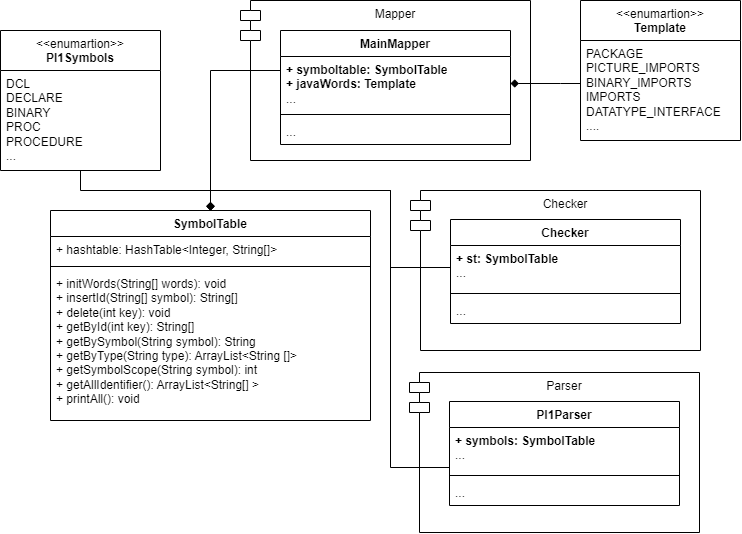
\includegraphics[scale=0.75]{symboltable-module-uml.drawio.png}
	\label{fig:symboltable}
\end{figure}

Das Modul \verb+Symboltable+ enthält die Klassen \verb+SymbolTable+, \verb+Pl1Symbols+ und \verb+PictureMapper+.
Zusätzlich enthält das Modul die Enums \verb+Pl1Symbols+ und \verb+Template+.

% Wie funktioniert SymbolTable und Pl1Smybols?
Die Klasse \verb+SymbolTable+ wird beim instanziieren des Objekts mit den Werten aus dem Enum \verb+Pl1Symbols+ inistallisiert. 
Bei der Datenstruktur der Symboltabelle handelt es sich um eine Hashtabelle. Ein Integer wird als Id verwendet und ein String Array um die Daten über die Variable bzw. das Wort zu Speichern. 
Wenn ein Bezeichner in die Symboltabelle eingefügt wird müssen, ein String für den Bezeichner, ein String für den Typ, ein Integer für die Sichtbarkeit und ein Integer für die Hierachiestufe der Variable hinterlegt sein. Nur so können andere Module wie der Parser, die Werte korrekt verarbeiten.
Der Parser verwendet die Symboltabelle etwa dazu, diese zu durchzuchen und um festzustellen ob der Wert bereits eingefügt wurde.
Dies kann der Fall sein, wenn der Bezeichner ein PL/I-Token ist oder während des übersetzens ein gleicher Wert eingefügt wurde.
Dann sollte die Methode, in der die \verb+insert+ Methode der \verb+Symboltable+ Klasse eine Fehlermeldung werfen.
Die Methode \verb+getSymbolScope+ wird dazu verwendet den Sichtbarkeitswert eines Bezeichners auszugeben. Das ermöglicht eine dedizierte,
abwägung wie dieser Wert verwendet werden soll. Diese Methode wird in dem Checker Modul in Kapitel ?.? erneut betrachtet.
Restliche Methoden sind hauptsächlich dazu da, Symbole gezielt abzufragen oder in der Konsole auszugeben.

% Wie funktioniert Template?
Der weitere Enum \verb+Template+ dient, in einem der folgenden Prozessschritte den Abstrakten-Syntax-Baum in Java-Code umzuwandeln.
In diesem Enum sind Java-Quellcode Ausschnitte hinterlegt die PL/I-Quellcode repräsentieren können. Sie werden in dem Mapper Modul verwendet
um nach und nach den Java-Zielcode zu erzeugen.

Um den Abstrakten Syntax Baum zu erzeugen muss der Parsebaum Stück für Stück überprüft werden. Dieser Prozess wird als semantische Analyse bezeichnet und erfolgt im Checker Modul.
 
\subsubsection{Checker}
Das Checker Modul prüft den Parsebaum auf seine korrektheit. Während des parsings wird etwa nicht der Typ von Variablen überprüft, wenn diese initalisiert werden. Weiterhin wird beim Parsing auch nicht überprüft ob eine Prozedur korrekt von dem \verb+begin+ und dem \verb+end+ ummantelt wird. Der Fehler in Listing ?.? wird durch den Parser alleine nicht erkannt.

\begin{verbatim}
proc_1: PROC;
	RETURN;
END proc_2;
\end{verbatim}

Zu erkennen ist das die Prozedur \verb+proc_1+ nicht equivalent mit dem selben Bezeichner schließt, sondern stattdessen, ein neuer Bezeichner eingefügt wird der aus diesem Kontext nicht verwendet wird.

% @todo UML-Diagramm Checker Modul


Um dieses Problem zu lösen wurde die Klasse \verb+ReferenceChecker+ implementiert. Die Klasse \verb+ReferenceChecker+, erbt so wie jede \verb+Checker+-Klasse von der Klasse \verb+Checker+.
Die Klasse \verb+Checker+ implementiert einen Depth-in-first Suchalgorhitmus um den Parse-Baum nach bestimmten Attributen der einzelnen Knoten zu durchsuchen, sowie gezielt nach bestimmten Knoten zu durchsuchen. Diese Methode ist neben der semantischen Analyse, auch für die Synthese des ASTs zu Java entscheidend. 
In Listing ?.? ist die beschriebene Methode gelistet.

\begin{verbatim}
protected void searchNode(SimpleNode root, String expectedNode) {
		if (root.jjtGetParent() == null) {
			stack.push(root.toString());
			if(isNode((SimpleNode)root, expectedNode)) {
				this.foundNodes.add(root);
			}
			
			if (this.hasChildren(root)) {
				for (int i = 0; i < root.jjtGetNumChildren(); i++) {
					stack.push(root.jjtGetChild(i).toString());
					
					if(isNode((SimpleNode)root.jjtGetChild(i), expectedNode)) {
						this.foundNodes.add((SimpleNode)root.jjtGetChild(i));
					}		
					searchNode((SimpleNode) root.jjtGetChild(i), expectedNode);
					stack.pop();
				}
			}
			else {
				return;
			}
		}
		else {
			if (root.jjtGetChild(0) == null && stack.getLast() == root.toString()) {
				stack.pop();
				return;
			}
			for (int i = 0; i < root.jjtGetNumChildren(); i++) {
				stack.push(root.jjtGetChild(i).toString());
				if(isNode((SimpleNode)root.jjtGetChild(i), expectedNode)) {
					this.foundNodes.add((SimpleNode)root.jjtGetChild(i));
				}
				if (this.hasChildren(root.jjtGetChild(i))) {
					searchNode((SimpleNode) root.jjtGetChild(i), expectedNode);
					stack.pop();
				}
				else {
					stack.pop();
				}
			}
		}
	}

\end{verbatim}

Die Methode in Listing ?.? arbeitet mit einem Stack. Immer wenn ein Knoten des Parsebaums aufgerufen wurde, wird das Knoten-Element in den Stack gelegt. Der Stack ist in der Klasse \verb+Stack+ implementiert. Der Knoten wird erst aus dem Stack entfernt, wenn auch alle Kindknoten eines Knotes erfasst wurden. 
Hat ein Knoten, Kindknoten wird die Methode Rekursiv aufgerufen und terminiert wenn ein Blatt der Parsebaums erreicht wurde.
Dieser Algorhitmus ermöglicht es im Zusammenhang mit der \verb+ReferenceChecker+ Klasse den Parsebaum nach etwaiigen \verb+END+ Knoten zu durchsuchen.
Hier wird dann das Attribut END Knotens abgefragt und mit dem Attribut des \verb+HEAD+ Knotens der zugehörigen Prozedur verglichen. Sind die Werte unterschiedlich wird eine Exception geworfen.

Neben einem Referenz-Fehler einer Prozedur-terminierung, gibt es, wie eingangs beschrieben auch Typ fehler bei der initalisierung die nicht von dem Parser erkannt werden können.
Da dies Teil der Semantik der Programmiersprache PL/I ist und nicht Teil der Syntaktik.
Der Ausdruck in Listing ?.? wird fälschlicherweise von dem Parser verarbeitet.

\begin{verbatim}
DCL var_1 DECIMAL(5);
var_1 = Hello;
\end{verbatim}

Um solche Semantischen Fehler zu erkennen, wird die Klasse \verb+TypeChecker+ implementiert. 
Auch diese Klasse ist eine Kindklasse der Checker-Klasse. Hier wird erneut der Depth-In-Frist Suchalgorhitmus verwendet um ein \verb+INIT+ Knoten zu finden. Dieser Knoten beinhaltet Informationen über die Variable die Initalisiert wurde und den Wert mit der sie initalisiert wurde.
 
Zusätzlich wird auch nach den \verb+VAR+ Knoten gesucht. Dieser Knoten beinhaltet durch seine Kindknoten Informationen über den Bezeichner der Variable und den Type.

Das Ergebnis beider Suchen wird je in eine Liste gespeichert. Schlussendlich werden die Typen und der initalisierte Wert miteinander verglichen. Liegt ein unzulässiger Wert vor wird eine entsprechende Exception geworfen.

Das Checker Modul bereitet den Parsebaum entsprechend so vor, dass dieser weiterhin in der Synthese verarbeitet werden kann. Erst nachdem die Semantische Analyse erfolgt ist handelt es sich um eine Zwischencode erzeugung. 
Nachdem also der Transpiler den PL/I-Quellcode in eine Zwischencode Erzeugung Umgewandelt hat, kann das Mapper-Modul mit der Synthese in Java-Zielcode beginnen.
 
\subsubsection{Mapper}
Das Mapper Modul transformiert die Zwischencode repräsentation in den Java-Zielcode. Dazu wurde das Mapper-Modul nachdem Strategy Desgin-Pattern entworfen.
In Abbildung ?.? ist das UML des Mapper Moduls zu sehen. 

\begin{figure}[h]
	\centering
	\caption{Mapper Modul}
	\includegraphics[scale=0.75]{mapper-module-uml.drawio.png}
	\label{fig:mapper}
\end{figure}

Die Klasse \verb+Mapper+ wird in der Main-Methode des Projektes instanziiert. Als Parameter wird der Wurzelknoten des Parssebaums übergegeben.
Woraufhin mithilfe der \verb+iterateParsetree+ Methode durch den Parsbaum iteriert wird. Hier wurde der Depth-in-first Suchalgorhitmus implementiert um
jeden Knoten zu verarbeiten. Jeder Knoten wird über seine zugehörige Identifaktionsnummer überprüft.  
In der Klasse \verb+AstMapper+ finden sich jegliche Identfikations-variablen der Knoten. Hier werden diese, mit den zugehörigen Mapper-Klasse in einer HashMap gespeichert.
Die Mapper Klassen, stellen die unterschiedlichen Strategien in dem Strategy-pattern dar. Sie implementieren alle das TranslationBehavior interface und 
aufgrunddessen eine \verb+translate+ Methode die den übersetzten Ausdruck zurückgibt. 

In der \verb+iterateParseTree+ Methode wird, für jeden Knoten überprüft ob eine solche Mapper-Klasse in der HashMap, der \verb+AstMapper+ Klasse vorhanden ist.
Falls eine Klasse vorhanden ist, wird in der TranslationBehavior Klasse, das entsprechende Strategie-Objekt des Typs \verb+TranslationBehavior+ in der
Mapper Klasse gesetzt. So wird die Translate-Methode der aktuell gesetzen Klasse aufgerufen und der Parsebaum-Knote in Java übersetzt.
Eine Mapper-Klasse kann weitere Methoden enthalten die, die Wahl des zu übersetzenden Ausdrucks entscheiden. Der Picture Mapper ist eine der Mapper-Klassen
um den Picture-Typ des ursprünglichen PL/I-Quellcodes zu übersetzen.

% wie funktioniert der PicturemMapper
Die Klasse \verb+PictureMapper+ enthält Zeichenkettenbeschränkungen des PL/I-Picture Typs und deren übersetzung als Regulären Ausdruck.
Da die Zeichenkettenbeschränkung aus PL/I nicht in dem Java Zielcode angewendet werden kann, werden die Ausdrücke entsprechend in Reguläre Ausdrücke übersetzt.
Mit der \verb+getRegex+ Methode der \verb+PictureMapper+ Klasse wird der übersetzte Reguläre Ausdruck als String zurückgegeben.
Der PL/I-Ausdruck \verb+(4)A+ wird etwa zu dem Regulären Ausdruck \verb+(A-Za-z ){4}+. In dem Java-Zielcode wurd zusätzlich eine Picture-Klasse implementiert,
die als Parameter den Regulären Ausdruck entgegennimmt und daraufhin über importierte Java-Klassen überprüft ob dieser den Bedingungen des Regulären Ausdrucks entspricht.  

Neben der PictureMapper Klassen, erzeugen weitere Mapper Klassen Stück für Stück den Java-Zielcode. 
Jegliche Ausdrücke werden am Ende in der Arraylist der Mapper Eltern-Klasse \verb+javaExpression+ gespeichert.
Wenn der Depth-in-first Algorhitmus jeden Knoten des Parse-Baums überprüft hat, wurde entweder das Programm erfolgreich übersetzt, oder während der Überpürufn 
eine Fehlermeldung geworfen.
Zu den Fehlermeldungen soll im folgenden Kapitel das Moudl Errorhandling vorgestellt werden.
Dieses dient hauptsächlich der Fehlerbehandlung und Fehlerinformation, für den Anwender.

\subsubsection{error-Handling}

\subsection{testing und Integration}
%1. transpiler wird getestet
%1.1 testen der methoden von Lexer, Parser usw. (Bsp.: Kann dieses Zeichen verarbeitet werden?)
%1.2 baum testen auf Korrektheit

%2. transpilieren wird getestet
%2.1 output des transpilierten Pl/1 Codes im Verhältnis zum Pl/1 Code testen.

%3. der transpilierte Code wird getestet
%- wie wird pl/1 Code Native getestet
%- funktioniert der Java Code richtig

%4. performance test (erst am ende)

\subsection{fehlerbehandlung}
um dem benutzer die Bediengung während der Laufzeit zu erleichtern, wurden Selbstgewählte Fehlermeldungen implementiert. Diese Fehlermeldungen sollen den Benutzer der Software in eine Feedback schleife bringe welche klare Anweisung zur Bediengung gibt. In der usprünglichen Version des Transpilers wurde dem Benutzer lediglich die von Java geworfenen Fehler in der Konsole ausgegeben. Die Fehlermeldung"IndexOutOfBounds", ließ dabei nicht darauf schließe das der Transpiler die PL/I Datei zum lesen nicht findet. Eine solche Fehlermeldung führt erneut dazu, dass der Benutzer sich selbst um die Lösung des Problems kümmern musste und somit einer weiteren Hürde begenete.
eben für dan fall das die Datei nicht gelesen werden kann, wurde eine Exception geschrieben. Die Exception "PliFileNotFound", beschreibt dem Benutzer die Ursache des Problems und nennt auch ein etwaaigen Lösungsvorschlag. Es exstieren in der neusten Version einige Exceptions die in der folgenden Tabelle näher Beschrieben werden.

...tabelle mit exceptions...

fehlerbehandlung spielt besonder im Zusammenhang mit der Lexikalischen Analyse eine Rolle. Um zu gewährleisten das die Transformation korrekt albläuft braucht es der formalen PL/I Grammatik enstrpechend richtigen PL/I Code als Eingabe. Eine nicht behandlung hätte zur Folge das das Programm entweder eine Fehlerhafte Ausgabe produziert, oder Fehlschlägt. Dies soll vermieden werden.

\section{technische Spezifikation}
	\subsection{Ausführung des Transpilers}
		\subsubsection{Transformationsmöglichkeiten}
		%Toleranzspielräume:...Einfach, Genau, Präzisse
		\subsubsection{Umwandlung von Datentypen}
		\subsubsection{Umwandlung von Prozeduren}
	\subsection{Optimierung}
	% online-Smoketest von PL/I Code -> %todo: Verschieben nach Erweiterbarkeit (Schlusskapitel), weil momentan noch nicht vollständige Grammatik realisiert.
	ein weiterer denkbarer Einsatzbereich ist es, den PL/I-Code auf seine Richtigkeit zu testen. Wird mithilfe des Programms erfolgreich das PL/I-Programm in Java übersetzt, so sollte auch ein herkömmlicher PL/I-Compiler auf einem Mainframe den Code ausführen können. Somit eignet sich das Programm auch für Smoke-tests von Anwendungen.
		\subsubsection{Performance und Benchmarks}
		\subsubsection{Testing}
